\documentclass[tikz,margin=0.6mm]{standalone}

% pdftk jigsaw.pdf burst  output jigsaw%d.pdf
% for i in {1..12}; do pdftocairo -singlefile -transp -r 350 -png jigsaw$i.pdf jigsaw$i; done

% pdftocairo -f 11 -l 11 -singlefile -transp -r 600 -png jigsaw.pdf jigsaw11

% pdftocairo -singlefile -transp -r 350 -png jigsaw1.pdf jigsaw1

\usepackage{amsmath}
\usepackage{amssymb}
\usepackage{physics} % \usepackage[arrowdel]{physics}
\usepackage{txfonts} % times for math (for consistency)
\usepackage{times}
\usepackage{jigsaw}

\usetikzlibrary{calc}

\gdef\sigb{\vb*{\sigma}}
\gdef\taub{\vb*{\tau}}
\gdef\epsb{\dot{\vb*{\epsilon}}}
\gdef\eps#1{\dot{\epsilon}_{#1}}
\gdef\statevec{\vb{s}}
\gdef\bulkvisc{\vb*{\eta}}
\gdef\bulkvisc{E_{ij}}

\gdef\Mmat{\vb{M}}

%\gdef\mygray{black!9!white}
\definecolor{mydarkgray}{RGB}{200,200,200} 
\definecolor{mygray}{RGB}{240,240,240} 

\definecolor{colorFL}{RGB}{198,219,239} % flow law 
\definecolor{colorMB}{RGB}{218,218,235} % momentum balance
\definecolor{colorFM}{RGB}{199,233,192} % fabric model
\definecolor{colorVA}{RGB}{253,208,162} % viscous anisotropy

\gdef\asp{0.75}
\gdef\asp{0.85}
\gdef\scale{2.0}

\gdef\mylarge#1{ #1 }
\gdef\mysmall#1{ {\fontsize{6.0}{6.0}\selectfont #1} }

%\gdef\textFL{\mylarge{$\taub(\epsb,\bulkvisc, \vb{m}_i, \cdots)$}}
%\gdef\textMB{}
%\gdef\textVA{}
%\gdef\textFM{\mylarge{$\dfrac{\mathrm{D} \statevec}{\mathrm{D} t} = \vb{M}\dotproduct\statevec$}}

\gdef\nameFM{CPO evolution}


\tikzset{every picture/.style={line cap=rect,line width=0.6pt}}

\newcommand{\blockFL}[1]{
	\begin{scope}[xshift=0cm,yshift=1cm]
	    \color{black}
	    \piece[#1]{1}{-1}{0}{0}
	    \color{black}    
	    \node at (0.5,0.55) {\mylarge{$\taub(\epsb,\bulkvisc, \vb{m}_i, \cdots)$}};
	    \node[anchor=west] (FL) at ({(0)},{(0.9)}) {\mysmall{Bulk rheology}};
	\end{scope}   
}

\newcommand{\blockMB}[1]{
\begin{scope}[xshift=1cm,yshift=1cm]
    \color{black}
    \piece[#1]{-1}{0}{0}{1}
    \color{black}    
    \node at (0.630,0.53) {\mylarge{$-\div\sigb=\rho\vb{g}$}};
    \node at (0.630,0.37) {\mylarge{$\sigb=\taub-p\vb{I}$}};
    \node[anchor=east] (MB) at ({(1)},{(0.9)}) {\mysmall{Momentum balance}};
\end{scope}   
}

\newcommand{\blockFM}[1]{
\begin{scope}[xshift=1cm,yshift=0cm]
    \color{black}
    \piece[#1]{0}{0}{1}{-1}
    \color{black}
	\node at ({0.5},0.45) {\mylarge{$\dfrac{\mathrm{D} \statevec}{\mathrm{D} t} = \Mmat\dotproduct\statevec$}};
    \node[anchor=east] (FM) at ({1},0.1) {\mysmall{\nameFM}};
\end{scope}    
}

\newcommand{\blockVA}[1]{
\begin{scope}[xshift=0cm,yshift=0cm]
    \color{black}
    \piece[#1]{0}{1}{-1}{0}
    \color{black}
	\node[align=left] at ({0.38},0.47) {\mylarge{$\bulkvisc(\statevec)$, $\vb{m}_i(\statevec)$}};
	\node[anchor=west,align=left] (VA) at ({0},0.10) {\mysmall{Viscous anisotropy}};
\end{scope}   
}

%%%%

\newcommand{\blockFLtext}[1]{
\begin{scope}[xshift=0cm,yshift=1cm]
    \color{black}
    \piece[#1]{1}{-1}{0}{0}
    \color{black}    
    \node[txtnode] at (0.5,0.6) {Bulk\\ rheology};
\end{scope}   
}

\newcommand{\blockMBtext}[1]{
\begin{scope}[xshift=1cm,yshift=1cm]
    \color{black}
    \piece[#1]{-1}{0}{0}{1}
    \color{black}    
    \node[txtnode] at (0.630,0.54) {Momentum\\ balance};
\end{scope}   
}

\newcommand{\blockFMtext}[1]{
\begin{scope}[xshift=1cm,yshift=0cm]
    \color{black}
    \piece[#1]{0}{0}{1}{-1}
    \color{black}
	\node[txtnode] at ({0.5},0.425) {CPO\\ evolution};
\end{scope}    
}

\newcommand{\blockVAtext}[1]{
\begin{scope}[xshift=0cm,yshift=0cm]
    \color{black}
    \piece[#1]{0}{1}{-1}{0}
    \color{black}
	\node[txtnode] at ({0.38},0.45) {Viscous\\ anisotropy};
\end{scope}   
}

%%%%

\usepackage{pgfplots}
\usetikzlibrary{patterns}
\usetikzlibrary{shapes}
\usetikzlibrary{backgrounds}
\usetikzlibrary{decorations.pathmorphing}
\usetikzlibrary{decorations.markings}
\usetikzlibrary{shadows} 

\definecolor{bgcolor}{HTML}{f7f6ee} % grayish

\tikzset{
	projboxtitle/.style={darkgray, line width=0.5pt, align=left, draw=gray, inner sep=0.9ex, font=\fontsize{5.0pt}{5.0pt}\selectfont, fill=bgcolor!50, }, % drop shadow={shadow xshift=0.6ex,shadow yshift=-0.6ex},
	projbox/.style={line cap=butt, align=left, yshift=-0.4em, xshift=1em,	darkgray, line width=2pt, font=\fontsize{9pt}{9pt}\selectfont, rectangle, },
}

\begin{document}

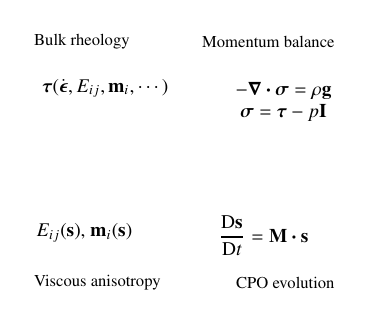
\begin{tikzpicture}[xscale=\scale,yscale={\scale*\asp}]
\scriptsize
\blockFL{colorFL}
\blockMB{colorMB}
\blockVA{colorVA}
\blockFM{colorFM}
\end{tikzpicture}

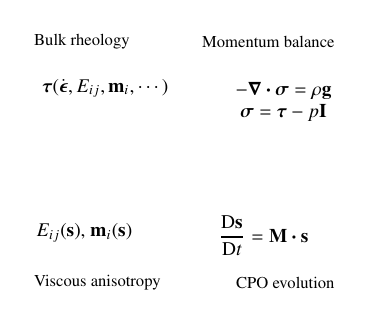
\begin{tikzpicture}[xscale=\scale,yscale={\scale*\asp}]
\scriptsize
\blockFL{mygray}
\blockMB{mygray}
\blockVA{mygray}
\blockFM{colorFM}
\end{tikzpicture}

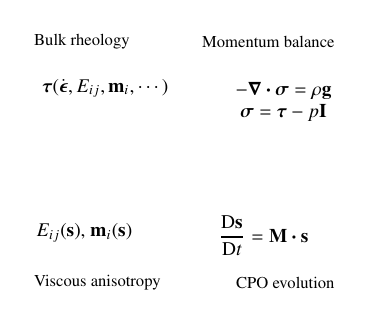
\begin{tikzpicture}[xscale=\scale,yscale={\scale*\asp}]
\scriptsize
\blockFL{mygray}
\blockMB{mygray}
\blockVA{colorVA}
\blockFM{mygray}
\end{tikzpicture}

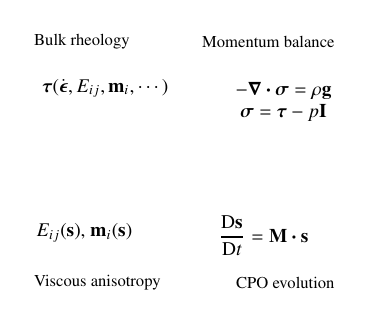
\begin{tikzpicture}[xscale=\scale,yscale={\scale*\asp}]
\scriptsize
\blockFL{colorFL}
\blockMB{mygray}
\blockVA{mygray}
\blockFM{mygray}
\end{tikzpicture}

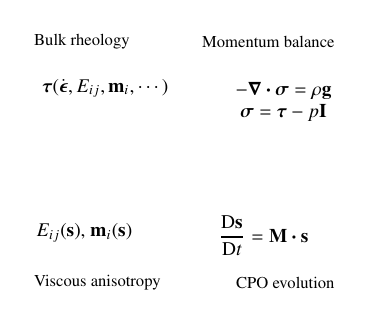
\begin{tikzpicture}[xscale=\scale,yscale={\scale*\asp}]
\scriptsize
\blockFL{mygray}
\blockMB{colorMB}
\blockVA{mygray}
\blockFM{mygray}
\end{tikzpicture}


%\begin{tikzpicture}[xscale=\scale,yscale={\scale*\asp}]
%	
%	\scriptsize
%	\blockFL{colorFL}
%	\blockMB{colorMB}
%	\blockVA{colorVA}
%	\blockFM{colorFM}
%
%	\gdef\litbox#1#2#3#4#5{
%		\node[projboxtitle] (#5) at (#1,#2) {#3};
%		\node[] (#5box) [projbox, anchor=north west] at (#5.south west) {#4};
%	}
%	
%	\litbox{4.8em}{-4.2em}{Placidi et al. (2006, 2009)\\ Richards et al. (2021)\\ Faria (2001, 2002, 2014) \\ Thorsteinsson et al. (2001, 2002, 2003) \\ Gagliardini and Meyssonnier (1999) \\ Gödert (2003) \\ Svendsen and Hutter (2006) \\ Kennedy et al. (2013, 2015) \\ Llorens et al. (2015) \\ \textit{... and more}}{}{FMbox}
%	
%	\litbox{-4.7em}{4.3em}{Gillet-Chaulet et al. (2005)\\ Staroszczyk and Gagliardini (1999) \\ Svendsen and Hutter (2006) \\ Pettit et al. (2007) \\ Azuma (1994, 1996)\\ Martin et al. (2009, 2014) \\ Hruby et al. (2020) \\ Ma et al. (2010) \\ Castelnau et al. (1996)\\ Gödert and Hutter (1998)\\ Gagliardini and Meyssonnier (1999)\\ Seddik et al. (2008) \\ Greve et al. (2008) \\ Thorsteinsson (2001, 2002) \\ Mangeney and Califano (1998) \\ \textit{... and more}}{}{FLbox}
%	
%	\gdef\arrlen{2em}
%	\draw[-latex, thick] (FM) to[bend left] (FMbox.50);
%	\draw[-latex, thick] (0,7.4em) to[bend right] (FLbox.38);
%	\draw[-latex, thick] (0,2.5em) to[bend left] (FLbox.334);
%
%\end{tikzpicture}

\gdef\txtscale{1.9}
\tikzset{
	txtnode/.style={align=center, font=\fontsize{7.3}{7.3}\selectfont}
}

\begin{tikzpicture}[xscale=1*\txtscale,yscale=0.8*\txtscale]
\blockFLtext{colorFL}
\blockMBtext{colorMB}
\blockVAtext{colorVA}
\blockFMtext{colorFM}
\end{tikzpicture}

\begin{tikzpicture}[xscale=1*\txtscale,yscale=0.8*\txtscale]
\blockFLtext{colorFL}
\blockMBtext{mygray}
\blockVAtext{mygray}
\blockFMtext{mygray}
\end{tikzpicture}

\begin{tikzpicture}[xscale=1*\txtscale,yscale=0.8*\txtscale]
\blockFLtext{mygray}
\blockMBtext{colorMB}
\blockVAtext{mygray}
\blockFMtext{mygray}
\end{tikzpicture}

\begin{tikzpicture}[xscale=1*\txtscale,yscale=0.8*\txtscale]
\blockFLtext{mygray}
\blockMBtext{mygray}
\blockVAtext{colorVA}
\blockFMtext{mygray}
\end{tikzpicture}

\begin{tikzpicture}[xscale=1*\txtscale,yscale=0.8*\txtscale]
\blockFLtext{mygray}
\blockMBtext{mygray}
\blockVAtext{mygray}
\blockFMtext{colorFM}
\end{tikzpicture}

\begin{tikzpicture}[xscale=1*\txtscale,yscale=0.8*\txtscale]

\blockFLtext{colorFL}
\blockMBtext{colorMB}
\blockVAtext{colorVA}
\blockFMtext{colorFM}

	\gdef\litbox#1#2#3#4#5{
		\node[projboxtitle] (#5) at (#1,#2) {#3};
		\node[] (#5box) [projbox, anchor=north west] at (#5.south west) {#4};
	}
	
	\litbox{9.2em}{1.7em}{Placidi et al. (2006, 2009)\\ Richards et al. (2021)\\ Faria (2001, 2002, 2014) \\ Thorsteinsson et al. (2001, 2002, 2003) \\ Gagliardini and Meyssonnier (1999) \\ Gödert (2003) \\ Svendsen and Hutter (2006) \\ Kennedy et al. (2013, 2015) \\ Llorens et al. (2015) \\ \textit{... and more}}{}{FMbox}
	
	\litbox{-3.5em}{2.6em}{Gillet-Chaulet et al. (2005)\\ Staroszczyk and Gagliardini (1999) \\ Svendsen and Hutter (2006) \\ Pettit et al. (2007) \\ Azuma (1994, 1996)\\ Martin et al. (2009, 2014) \\ Hruby et al. (2020) \\ Ma et al. (2010) \\ Castelnau et al. (1996)\\ Gödert and Hutter (1998)\\ Gagliardini and Meyssonnier (1999)\\ Seddik et al. (2008) \\ Greve et al. (2008) \\ Thorsteinsson (2001, 2002) \\ Mangeney and Califano (1998) \\ \textit{... and more}}{}{FLbox}
	
	\gdef\arrlen{2em}
	\draw[-latex, thick] (FM.18) to[bend left] (FMbox.199);
	\draw[-latex, thick] (0,4.8em) to[bend right] (FLbox.38);
	\draw[-latex, thick] (0,1.2em) to[bend right] (FLbox.330);

\end{tikzpicture}


\gdef\statevec{\vb{s}_k}
\gdef\Mmat{\vb{M}_k}
%\gdef\Mmat{\vb{M}_k(\grad \vb{u})}
\gdef\nameFM{CPO evolution}
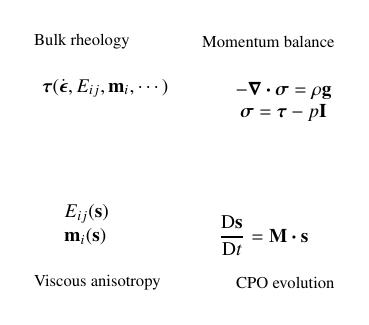
\begin{tikzpicture}[xscale=\scale,yscale={\scale*\asp}]
\scriptsize
\blockFL{colorFL}
\blockMB{colorMB}

\begin{scope}[xshift=0cm,yshift=0cm]
    \color{black}
    \piece[colorVA]{0}{1}{-1}{0}
    \color{black}
	\node[align=left] at ({0.38},0.53) {\mylarge{$\bulkvisc(\statevec)$\\[0.1em] $\vb{m}_i(\statevec)$}};
	\node[anchor=west,align=left] (VA) at ({0},0.10) {\mysmall{Viscous anisotropy}};
\end{scope}   

\blockFM{colorFM}

\end{tikzpicture}


%\begin{tikzpicture}[xscale=\scale,yscale={\scale*\asp}]
%
%\scriptsize
%\blockFL{colorFL}
%\blockMB{colorMB}
%\blockVA{colorVA}
%\blockFM{colorFM}
%
%%\gdef\box#1#2{
%%	\node[projboxtitle] (WPtitle) at (#1,#2) {#3};
%%	\node (WP) [projbox, anchor=north west] at (WPtitle.south west) {#4};
%%}
%
%\node[] (Eij) at ($(FM)+(-10em,-10em)$) {\includegraphics[scale=0.54,page=2]{../orthotropic/orthotropic.pdf}};
%\draw[-latex, thick] (VA) to[bend left] (Eij);
%
%\node[] (Eca) at ($(Eij)+(0.5em,+6em)$) {\includegraphics[scale=0.38,page=4]{../tranisotropic/tranisotropic-monocrystal.pdf}};
%
%
%
%\node[] (harmexp) at ($(FM)+(4em,-7em)$) {\includegraphics[scale=0.435]{../harmonic-expansion/harmonic-expansion-L2.pdf}};
%%\node[] at (harmexp)
%\draw[-latex, thick] (FM) to[bend left] (harmexp);
%
%
%\end{tikzpicture}

\end{document}
